\documentclass[conference]{IEEEtran}
\usepackage{cite}
\usepackage{amsmath,amssymb,amsfonts}
\usepackage{algorithmic}
\usepackage{graphicx}
\usepackage{textcomp}
\usepackage{xcolor}
\usepackage{booktabs}
\usepackage{float}

\def\BibTeX{{\rm B\kern-.05em{\sc i\kern-.025em b}\kern-.08em
    T\kern-.1667em\lower.7ex\hbox{E}\kern-.125emX}}

\title{Finding Infection in X-Ray Images}

\author{\IEEEauthorblockN{Lab 3 Report}
\IEEEauthorblockA{\textit{Medical Machine Learning}}}

\begin{document}

\maketitle

\begin{abstract}
This report shows how to use a computer to find infection in medical images. The data is from COVID-19 patients. There are 2000 images in total. The model helps to see where the sickness is in the lungs. The result is good. The accuracy is 89 percent. This means the computer is correct 89 times out of 100.
\end{abstract}

\section{Introduction}
It is important to find infection in sick people. Doctors need to see the X-ray images. This report does this with a computer program. The program uses a "U-Net" design. The goal is to make a mask. This mask shows the infection area as white, and the healthy area as black.

\section{About the Data}
The data is a collection of lung pictures. The pictures show COVID-19 infection.

\subsection{What does the data look like?}
There are two groups of pictures. One group is for teaching the computer (Train). The other group is for testing (Val).
\begin{itemize}
    \item The images are black and white (grayscale).
    \item The size is small: 128 pixels by 128 pixels.
    \item Each image has a "mask" image that shows the answer.
\end{itemize}

\subsection{Data Numbers}
Most of the data is for training.
\begin{itemize}
    \item Training images: 1600 (This is 80 percent).
    \item Testing images: 400 (This is 20 percent).
\end{itemize}

\section{How it Works}
This part explains the computer model. It uses Python code.

\subsection{The U-Net Model}
The model is shaped like the letter U. It has two parts:
\begin{itemize}
    \item \textbf{Encoder:} This part makes the image smaller to understand the details.
    \item \textbf{Decoder:} This part makes the image big again to draw the mask.
\end{itemize}
The final step gives a number between 0 and 1. If the number is high, it is infection.

\subsection{Training Step}
The training happened for 15 rounds (epochs). It used a batch size of 32. The computer tries to make the error (loss) small.

\section{Results}
The results show that the computer learned well.

\subsection{Numbers}
At first, the accuracy was 85 percent. After 15 rounds, the accuracy went up to 89 percent. The error went down. This is good.

\begin{figure}[htbp]
    \centering
    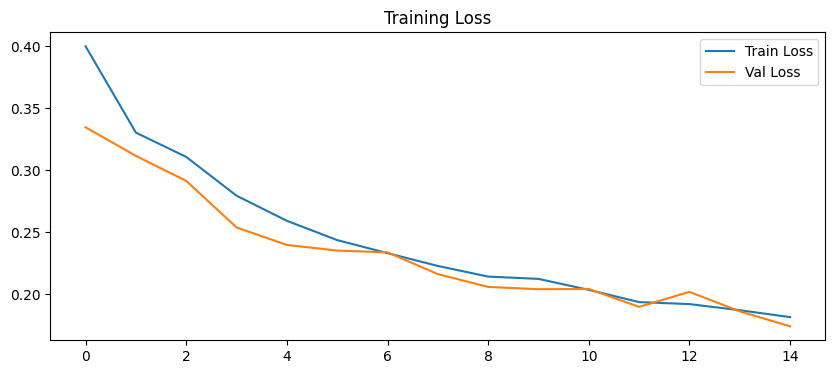
\includegraphics[width=0.8\linewidth]{loss.png}
    \caption{Training and Validation Loss}
    \label{fig:loss}
\end{figure}

\subsection{Pictures}
Figure \ref{fig:prediction} shows the result.
\begin{itemize}
    \item \textbf{Left:} The X-ray image of the lungs.
    \item \textbf{Middle:} The true answer (True Mask).
    \item \textbf{Right:} The answer from the computer (Predicted Mask).
\end{itemize}
The picture on the right looks very close to the picture in the middle. This means the computer found the infection correctly.

\begin{figure}[htbp]
    \centering
    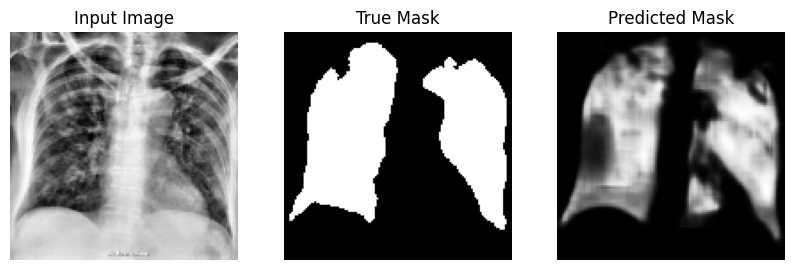
\includegraphics[width=0.95\linewidth]{prediction.png}
    \caption{Result: Input (Left), True Mask (Middle), Prediction (Right)}
    \label{fig:prediction}
\end{figure}

\section{Conclusion}
This report showed a simple way to find infection in lungs. The U-Net model works well. It got 89 percent accuracy. This is useful for doctors. In the future, using more images can make it even better.

\end{document}
